\documentclass{standalone}
\author{Quinten Bruynseraede}
\usepackage{tikz}
\usetikzlibrary{shapes}
\title{Tikz grafen}
\begin{document}\pagestyle{empty}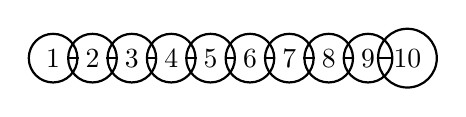
\begin{tikzpicture}\node[shape=circle,draw=black,align=center,line width=0.8pt] (0) at (0.5,10.166666666666666) {1};
\node[shape=circle,draw=black,align=center,line width=0.8pt] (1) at (1.0,10.166666666666666) {2};
\node[shape=circle,draw=black,align=center,line width=0.8pt] (2) at (1.5,10.166666666666666) {3};
\node[shape=circle,draw=black,align=center,line width=0.8pt] (3) at (2.0,10.166666666666666) {4};
\node[shape=circle,draw=black,align=center,line width=0.8pt] (4) at (2.5,10.166666666666666) {5};
\node[shape=circle,draw=black,align=center,line width=0.8pt] (5) at (3.0,10.166666666666666) {6};
\node[shape=circle,draw=black,align=center,line width=0.8pt] (6) at (3.5,10.166666666666666) {7};
\node[shape=circle,draw=black,align=center,line width=0.8pt] (7) at (4.0,10.166666666666666) {8};
\node[shape=circle,draw=black,align=center,line width=0.8pt] (8) at (4.5,10.166666666666666) {9};
\node[shape=circle,draw=black,align=center,line width=0.8pt] (9) at (5.0,10.166666666666666) {10};

\path [-,draw=black,line width=0.8pt] (0) edge node {} (1);
\path [-,draw=black,line width=0.8pt] (1) edge node {} (2);
\path [-,draw=black,line width=0.8pt] (2) edge node {} (3);
\path [-,draw=black,line width=0.8pt] (3) edge node {} (4);
\path [-,draw=black,line width=0.8pt] (4) edge node {} (5);
\path [-,draw=black,line width=0.8pt] (5) edge node {} (6);
\path [-,draw=black,line width=0.8pt] (6) edge node {} (7);
\path [-,draw=black,line width=0.8pt] (7) edge node {} (8);
\path [-,draw=black,line width=0.8pt] (8) edge node {} (9);
\end{tikzpicture}
\end{document}